\documentclass{article}
\usepackage[utf8]{inputenc}
\usepackage{hyperref}
\usepackage{graphicx}
\usepackage{float}
\usepackage{listings}

\title{Assignement 3}
\author{Iván Piña Arévalo \\ ivan.pinaarevalo@alum.uca.es}
\date{\today}

\begin{document}
\maketitle

\newpage
\begin{abstract}
    In this practice, we will make polynomial reduction implementation. Specifically oder in particular,
    we will reduce the coloured graph to the 3-SAT problem. Once implemented our problem, we will make 
    analysis about  temporal complexity, as well as relations between the number of colors required and the 
    Maximum Click of the graph. The Petersen graph has been used.  
\end{abstract}

\newpage

\section{Introduction}
First, we start talking about coloring of graph. This problem consists in coloring a graph in such a way 
that two adjacent vertices cannot have the same color.
    \begin{figure}[H]
        \centering
        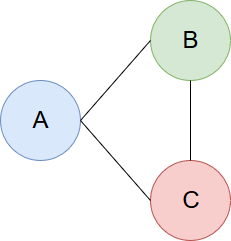
\includegraphics[width=0.5\textwidth]{pictures/ejemplo.png}
        \caption{Example with a valid solution.}
    \end{figure}
	
    \begin{figure}[H]
        \centering
        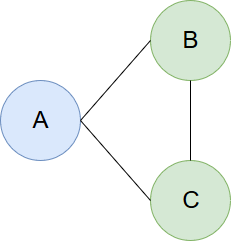
\includegraphics[width=0.5\textwidth]{pictures/ejemplobad.png}
        \caption{Example graph with a invalid solution}
    \end{figure}

    In particular, we had used the Peterson graph. We have slightly varied the numberin of nodes. For 
    convenience, the first node having been numbered "1", instead of "0" and so on (in other words, we 
    have increased to 1 the value of each node).

    \begin{figure}[H]
        \centering
        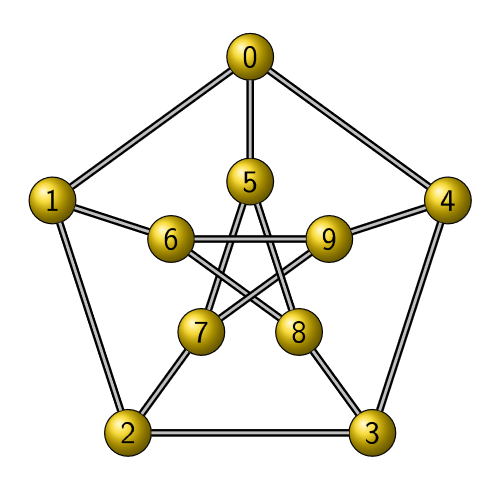
\includegraphics[width=0.5\textwidth]{pictures/PetersenGraph.png}
        \caption{Petersen Graph}
    \end{figure}

    To find the solution of this problem, has been used the 3-SAT problem. 
    The SAT problem was one of the first to discover NP-complet.
    This problem consists of given a Boolean equiation, finding the values for 
    which it is true. In addition, the equiation must have the following characteristics:
 
    \begin{itemize}
        \item The global equation is composed of equiations linked to the logical gate AND.
        \item Each subequation is composed of variables  ($x_1, x_2, ...$) joined by the logical door OR.
    \end{itemize}

    Below we can see an equation for the SAT problem:
        \[ ( x_1 \vee x_2 \vee x_3) \wedge (x_3 \vee x_4)\]

    
\section{Methodology}
All implementations have been made in C++, we have divided the problem into several parts.
    \subsubsection{Reading of the graph.}
    For the reading of the graph we have relied on a file. This file must have the following structure:
        \begin{itemize}
            \item The definition of each node is done in a row.
            \item The nodes to which the node we ar defining is connected are separated by commas.
        \end{itemize}
        
        In this way we perform the reading of the graph, represented by adjacency lists. Next we can 
        see the file wiht the example graph of the previous section.
        %Insertar fichero con el grafo de ejemplo.
        \begin{figure}[H]
            \centering
            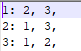
\includegraphics[width=0.2\textwidth]{pictures/entrada_ejemplo.png}
            \caption{Input file for the example graph}
        \end{figure}

        Similarly, the Petersen graph represented by adjacency lists. 
        \begin{figure}[H]
            \centering
            \includegraphics[width=0.2\textwidth]{pictures/petersen_modificado.png}
            \caption{Input file for the Petersen graph}
        \end{figure}
    
    \subsubsection{Transformation 3-Col to SAT}
    The first thing to do in this part was to deeply analyze the structure of the 
    Boolean equiations that represent the graph we want to color. These equations can be divided into two groups.
        \begin{itemize}
            \item Equations corresponding to the color of the node itself.
            \item Equations corresponding to the color of the nodes adjacent to the current node.
        \end{itemize}
        %Remarcar que por eficiencia temporal las aristas se escriben dobles, cosa que no afecta a picosat.
        If we look at the graphs we have used the edges are bidirectional. It would suffice to define them only once, 
        however, to mantain the readability of the code I have decided to allow them to be written twice (one in each direction). 
        This increase in number of equations does not affect PicoSAT. Next we show the output for the Petersen graph.
        %Insertar imagen grafo Petersen.
    
    \subsubsection{Writing boolen equations}
        Finally, it is necessary to write in a file the equations corresponding to the graph. These equations should be in DIMACS format. 
        The purpose of this format is the correct processing by the PicoSAT program.

        Simply instead of showing the equations by the standard output we have directed them towards a string. 
        We have also defined a variable that is responsible for counting how many equations it has and another 
        variable for the number of variables. Turning the strings and the counters in a file we get to have the information ready 
        for PicoSAT.

        The program has been parametrized in such a way that both the graph and the number of colors can be modified.  
    
    \subsubsection{PicoSAT}
        Finally, to execute the program we have used the orde: \\
         \vspace{5mm} $./picosat$ salida \\

        Si deseamos ver todas las soluciones \\
         \vspace{5mm} $./picosat$ --all salida


\section{Results and Discussion}
    To find out the type of reduction obtained, we have made a study of the temporal complexity 
    of the 3SAT program (that is, assuming the number of colors is 3). 
    \begin{figure}[H]
        \centering
        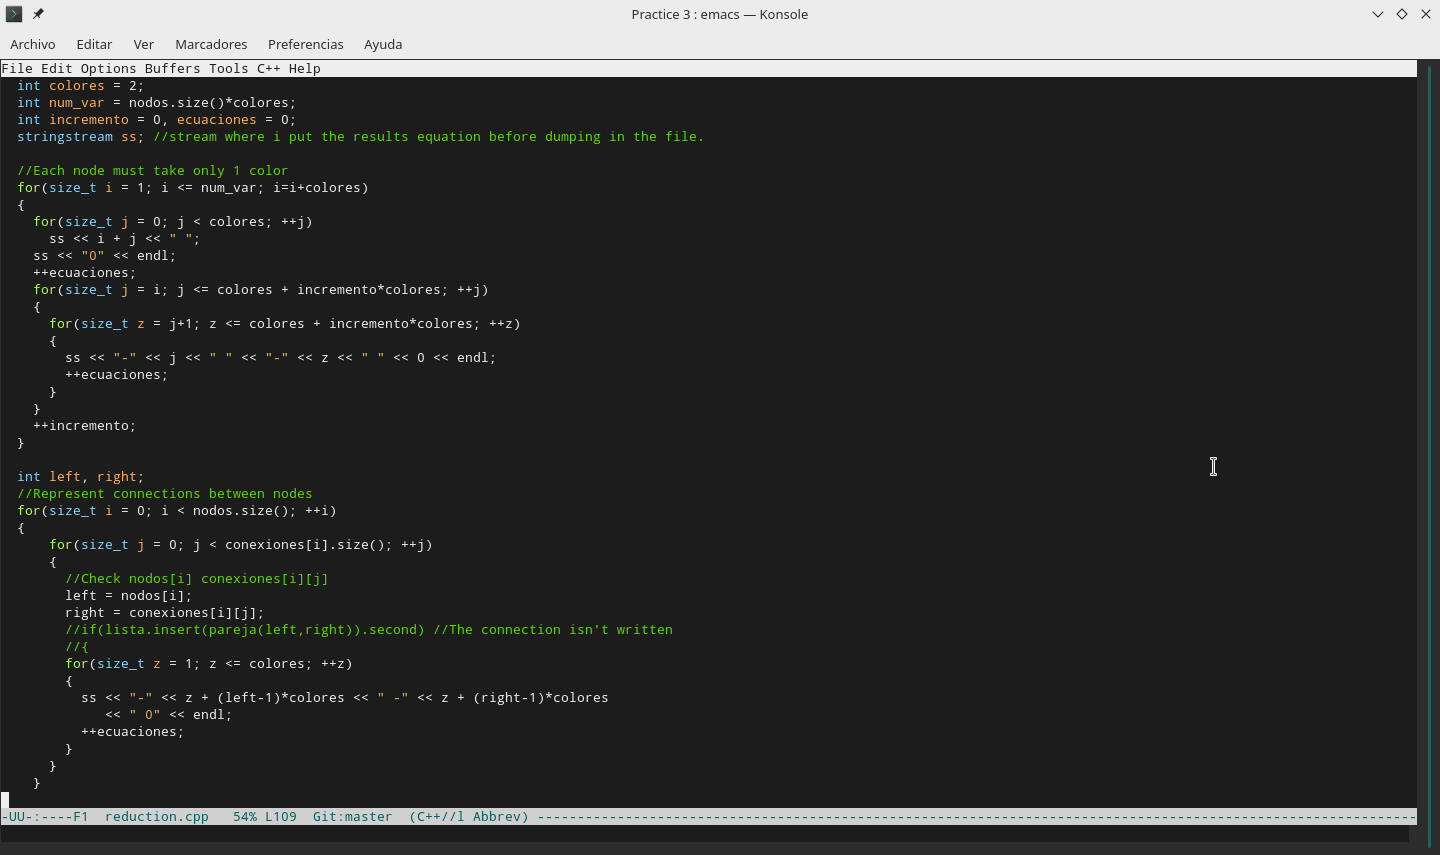
\includegraphics[width=1\textwidth]{pictures/analisis.png}
        \caption{Temporal analysis of the algorithm}
    \end{figure}
    As you can see, there are two nests of for loops. Therefore, we have decided to 
    divide in analysis into two blocks, each corresponding to a block of for loops. 

    Analyzing the behavior of the loops, we see tat the number of iterationes depends on two factors:
    \begin{itemize}
        \item Number of nodes: n.
        \item Number of colors: in this case it is 3.
    \end{itemize}

    At first nesting we distinguish 4 loops for:
    \begin{itemize}
        \item for(size\_t i = 1; i $\leq$ num\_var; i = i + colores): this loop is executed n times.
        \item for(size\_t j = 0; j $<$ colores; ++colores): this loop is executed colors times
        \item for(size\_t j = 0; j $\leq$ colores + incremento*colores; ++j): this loop is executed colors times
        \item for(size\_t z = j+1; z $\leq$ colores + incremento*colores; ++z): this loop is executed j-1 times
    \end{itemize}
    
    Therefore, the complexity of the first part is: 
    \[t(n) = n(3+3*1) = n\]
    We now analyze the second part of the algorithm. We distinguish the following loops:
    \begin{itemize}
        \item for(size\_t i = 0; i < nodos.size(); ++i): it is executed n times.
        \item for(size\_t j = 0; j < conexiones[i].size(); ++j): it is executed as many times as edges have the graph. In the worst case (n-1) times.
        \item for(size\_t z = 1; z <= colores; ++z): it is executed 3 times.
    \end{itemize}
    
    Therefore, the compexity of the second part is:
    \[t(n) = n((n-1)*3) = n^2\]
    
    Fusionando ambas partes, por la regla del máximo tenemos que el algoritmo tiene un orden $O(n) = n^2$, es decir, posee un orden polinómico. 
    Nuestro programa posee una complejidad polinómica. Consecuentemente hemos obtenido una reducción polinómica.

    %Insertar fichero de ecuaciones. 
    
    A solution for the Peterson graph with three colors is this:
    \begin{figure}[H]
            \centering
            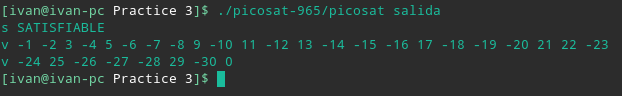
\includegraphics[width=0.8\textwidth]{pictures/solution.png}
            \caption{Solution for the Petersen graph}
        \end{figure}
        
    Likewise, two solutions are: 
    %Insertar la solución de las ecuaciones booleanas, no te compliques coloreando el grafo.
    \begin{figure}[H]
            \centering
            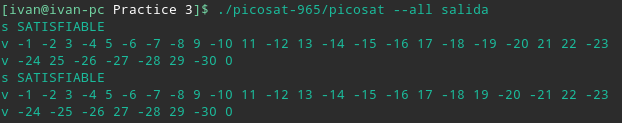
\includegraphics[width=0.8\textwidth]{pictures/solution_all.png}
            \caption{Two solutions for the Petersen graph}
    \end{figure}
        
    On the other hand, there is no solution if we decrease the number of colors to 2. Finally, 
    analyzing the structure of the graph we have that the Maximum Clique of the graph of Petersen is of size 2.
 
 

    The Maximum Clique of the graph is 2.  Furthermore we can not color the graph with less than three colors. This, intuitively suggests that:
    \[clique < numero\_colores\]

    By clique the number of nodes that form the maximum clique and number\_colors the minimum number needed to color the graph. 
    Now in order to contrast this assumption, we decided to try the sample graph we have shown at the beginning of the report
    %Insertar imagen 
    \begin{figure}[H]
        \centering
        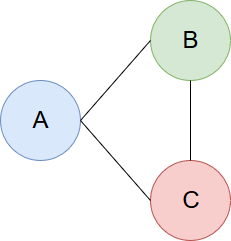
\includegraphics[width=0.5\textwidth]{pictures/ejemplo.png}
        \caption{Example graph}
    \end{figure}

    Here, however, the maximum clique of the graph is 3 and it can be colored correctly with three colors. Therefore we have to:
    \[clique \leq numero\_colores\]
    
    Consequently, we made an attemplt to color the Petersen graph with two colors
    \begin{figure}[H]
        \centering
        \includegraphics[width=0.5\textwidth]{pictures/interior.png}
        \caption{Interior del grafo de Petersen}
    \end{figure}

    It was not necessary to color the whole graph, working only with the inside we can see that it is not colorable with only 
    two colors, the  node number 9 can not take neither red nor green.   


\section{Conclussion}
As we have been able to verify, a polinomic reduction of the problem of the coloring of a graph to SAT can be realized. 
This fact states that the NP-Complete problems contain all the problems belonging to the NP class.

On the other hand, regarding the relation between the Clique and the maximum number of colors, it is concluded that not 
only the Clique influences the maximum number of colors needed. So does the structure of the graph. If we want to stick 
strictly to the Clique to estimate the number of colors, we have to: 
    \[clique < numero\_colores \] 

Although in some cases, when the structure of the graph allows it, it is possible that be fulfilled oder be accomplished: 
    \[clique \leq numero\_colores\]

    Consequently, if there was a Clique of size 4 in the graph, it would not be possible to color the graph with only 3 colors. 
    This fact is easily reasonable, on the other hand since if there is a Clique of size 4, there are vertexes (al least 4), which will have three adjacent vertexes.

\section{Bibliografia}
\begin{itemize}
    \item Kleinberg, Jon; Tardos, Éva Tardos (2006). Algorithm Design. Pearson Education. pp. 452–453. ISBN 978-0-321-37291-8.
    \item Goldreich, Oded (2008), Computational Complexity: A Conceptual Perspective, Cambridge University Press, pp. 59–60, ISBN 9781139472746
    \item  Garey, Michael R.; Johnson, D. S. (1979), Computers and Intractability: A Guide to the Theory of NP-Completeness, W. H. Freeman
\end{itemize} 

\end{document}
